
\subsection*{1.}

\(p(\overline{D}) = 1 - p(D) = 1 - \dfrac{2}{3} = \dfrac{1}{3}\).

\subsection*{2.}

\begin{center}
\begin{tikzpicture}[thick, scale=1.5] %{,}
\node (P_-1_0) at (-2,-1.5) {$\phantom{A}$};
\node (P_0_0) at (0,-0.5) {$D$};
\draw (P_-1_0) -- (P_0_0) node[midway, above] {$\dfrac23$};
\node (P_1_0) at (2,-0) {$S$};
\draw (P_0_0) -- (P_1_0) node[midway, above] {$\dfrac{9}{10}$};
\node (P_1_1) at (2,-1) {$\overline{S}$};
\draw (P_0_0) -- (P_1_1) node[midway, below] {$\dfrac{1}{10}$};
\node (P_0_2) at (0,-2.5) {$\overline{D}$};
\draw (P_-1_0) -- (P_0_2) node[midway, below] {$\dfrac13$};
\node (P_1_2) at (2,-2) {$S$};
\draw (P_0_2) -- (P_1_2) node[midway, above] {$\dfrac34$};
\node (P_1_3) at (2,-3) {$\overline{S}$};
\draw (P_0_2) -- (P_1_3) node[midway, below] {$\dfrac14$};
\end{tikzpicture}
\end{center}

\subsection*{3.}

\(p(\overline{D} \cap S) = p(\overline{D}) \times p_{\overline{D}}(S) = \dfrac{1}{3} \times \dfrac{3}{4} = \dfrac{1}{4}\).

\subsection*{4.}

D'après la loi des probabilités totales :
\begin{align*}
p(S) &= p(D \cap S) + p(\overline{D} \cap S) \\
&= \dfrac{2}{3} \times \dfrac{9}{10} + \dfrac{1}{4} \\
&= \dfrac{3 \times 4 + 1 \times 5}{4 \times 5} \\
&= \dfrac{17}{20} \\
&= 0{,}85.
\end{align*}

\subsection*{5.}

On calcule :
\[
p_S(\overline{D}) = \dfrac{p(S \cap \overline{D})}{p(S)} = \dfrac{p(\overline{D} \cap S)}{p(S)} = \dfrac{\dfrac{1}{4}}{\dfrac{3}{5}} = \dfrac{5}{12}.
\]

